\documentclass{IEEEtran}

\usepackage{graphicx}
\usepackage{caption}
\usepackage{subcaption}
\usepackage{hyperref}
\usepackage{url}

\begin{document}

\title{Computational Psycholinguistics --- Assignment 1}
\author{Daan Brugmans (S1080742)}
\date{\today}

\maketitle

This report is an extension of the code produced for the assignment.
This code comes in the form of a single Jupyter notebook, handed over alongside this report, and is also available at the following URL: \url{https://github.com/daanbrugmans/ru-computational-psycholinguistics-23-24/blob/main/assignment-1/main.ipynb}.
A \textit{requirements.txt} file is also provided for easy installation of the necessary libraries.
Although this report contains the most relevant results for the purpose of the assignment, some will not be included, and are exclusive to the notebook.

\section{Methodology}
For this assignment, two fully prepared test sets of primes, targets, and reaction times were handed to us, of which students should use one.
I use the "data naming" test set.
Although the data has already been fully cleaned and prepared, I apply some additional data preprocessing.
First, I set the semantic relatedness of unrelated prime-target pairs to a single class, \texttt{unrel}, as opposed to having two classes for unrelated prime-target pairs that have either low (\texttt{unrel\_strong}) or high (\texttt{unrel\_strong}) semantic similarity.
I made this choice because we want to analyze all unrelated prime-target pairs as a single, cohesive unit for the purposes of this assignment.
I also manually calculate the semantic priming effect.
I do this by comparing the difference between the mean reaction times of a specific target word for primes that are semantically related versus primes that are semantically unrelated.
I have made two design decisions here:
\begin{enumerate}
    \item I take the median of the related and unrelated mean reaction times, as opposed to calculating the mean or something else.
    This is because the final mean of the mean reaction times given per semantic relatedness category was quite sensitive to outliers, and I expected the median to be more representative of the data.
    \item I set all negative semantic priming effects to 0.
    This is because I calculate the difference by subtracting the median reaction time for related primes from the median reaction time for unrelated primes.
    If this value is negative, then that would imply that reaction times are actually faster when primes are unrelated.
    In this case, no semantic priming effect would be taking place, so I set it to 0.
\end{enumerate}

\begin{figure*}
    \centering
    \begin{subfigure}{0.4\textwidth}
        \centering
        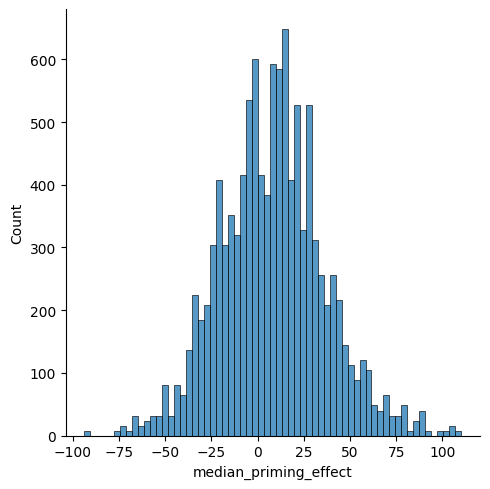
\includegraphics[width=\textwidth]{images/distribution_semantic_priming_effect_unnormalized.png}
        \caption{A plot of the distribution of semantic priming effects.}
        \label{fig:semantic_priming_unnormalized}
    \end{subfigure}
    \begin{subfigure}{0.4\textwidth}
        \centering
        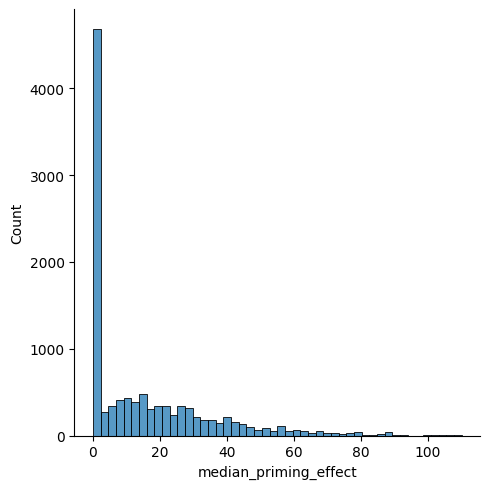
\includegraphics[width=\textwidth]{images/distribution_semantic_priming_effect_normalized.png}
        \caption{A plot of the distribution of semantic priming effects where all negative values have been set to 0.}
        \label{fig:semantic_priming_normalized}
    \end{subfigure}
    \caption{Distributions of the semantic priming effect.}
\end{figure*}

As part of the assignment, students should train multiple word2vec models, and use them in their analyses.
Specifically, students should pick two of three hyperparameters, those being model architecture, semantic embedding size, and word window size, and try out multiple values.
I have chosen to try out various values of the architecture (\texttt{sg}), that is, Continuous Bag-Of-Word (CBOW) models versus SkipGram models, and three different word window sizes (\texttt{window}): 2 (small), 5 (default), and 8 (large).
I was interested in these hyperparameters specifically, because I was did not know if a CBOW architecture would outperform a SkipGram architecture or vice versa, and I wanted to know how window size effected a model's ability to learn semantic representations.
I set the semantic embedding size (\texttt{vector\_size}) to a constant 300 dimensions, and train for 5 epochs.
I have saved the models and they can be found in the \texttt{models} folder at the following URL: \url{https://github.com/daanbrugmans/ru-computational-psycholinguistics-23-24/tree/main/assignment-1/models}.
If you download these models and put them in a folder called "models" in the same directory as the notebook, you should be able to use them.

For the purposes of the assignment, I perform two analyses:
\begin{enumerate}
    \item I compute the mean cosine similarity between prime-target pairs for all three semantic relatedness levels (strong, weak, unrelated), and compare their values to the semantic relatedness level.
    We expect to see that the mean cosine similarity should be higher in prime-target pairs that are semantically related than those that are not, since the cosine similarity between semantic embeddings is a measure of how closely related the semantics of two words are.
    \item I analyze the predictive power of the cosine similarity between prime-target pairs on the sizes of the priming effects.
    I do this by plotting the cosine similarities between prime-target pairs against the median priming effects I calculated.
    I also calculate a linear regression model of this relationship to quantitatively express that predictive power.    
\end{enumerate} 
I perform these analyses using six different word2vec models.

For the implementation of these analyses, I have constructed a handful of functions that encapsulate the analyses' steps:
\begin{itemize}
    \item calculate\_cosine\_similarities: calculates the cosine similarities of all prime-target pairs in the dataframe provided using the provided word2vec model.
    If the prime or target does not exist in the model's vocabulary, and thus cannot be modeled in the model's space, the cosine similarity is set to 0.
    This means that I assume that words are not semantically related at all if at least one of them is unknown to the word2vec model.
    \item print\_mean\_cosine\_similarity\_by\_semantic\_relatedness: calculates, then prints the mean cosine similarity for the three semantic relatedness levels (strong, weak, unrelated) using the provided dataframe and the specified cosine similarity column to use.
    \item plot\_cosine\_similarity\_as\_predictor\_of\_reaction\_time: paints the scatter plot of the cosine similarity of prime-target pairs against their mean reaction times, for every semantic relatedness level.
    It also calculates and paints a linear regression model for every scatter plot.
    This function is supplementary and shows how the cosine similarities are distributed among semantic relatedness levels, and how this distribution interacts with the distribution of mean reaction times.
    \item plot\_cosine\_similarity\_as\_predictor\_of\_priming\_effect: paints the scatter plot of the cosine similarity of prime-target pairs against their median priming effects.
    It also calculates and paints a linear regression model for the plot.
\end{itemize}

\section{Results}
Before training the models, I perform some data exploration. 
Specifically, I draw 2 plots: both of the distribution of the semantic priming effect, with plot \ref{fig:semantic_priming_unnormalized} including negative priming effects, and plot \ref{fig:semantic_priming_normalized} setting all negative priming effects to zero.
Although I only use the latter distribution in my analyses, the former distribution shows that, if unnormalized, the calculated semantic priming effects are normally distributed, centering around 0.
This would imply that more clearly noticeable instances of the semantic priming effect occur less often than hardly noticeable ones.

\begin{table}
    \centering
    \begin{tabular}{c|c|c|c}
        & \textbf{Strong} & \textbf{Weak} & \textbf{Unrelated} \\
        \hline \hline
        \textbf{CBOW Window 2} &0.410 &0.300 &0.077 \\
        \textbf{CBOW Window 5} &0.416 &0.305 &0.070 \\
        \textbf{CBOW Window 8} &0.415 &0.304 &0.065 \\
        \textbf{SkipGram Window 2} &0.397 &0.297 &0.113 \\
        \textbf{SkipGram Window 5} &0.410 &0.307 &0.105 \\
        \textbf{SkipGram Window 8} &0.417 &0.314 &0.107 
    \end{tabular}
    \caption{A table containing the mean cosine similarities for the three levels of semantic relatedness for all models trained.}
    \label{tab:mean_cosine_similarity_by_semantic_relatedness}
\end{table}

The results of the first analysis can be found in table \ref{tab:mean_cosine_similarity_by_semantic_relatedness}.
From these results, I find that, regardless of model architecture or window size, the mean cosine similarities for the semantic relatedness levels are all very similar: the mean for strong relatedness is always roughly 0.41, the mean for weak relatedness is always roughly 0.3, and the mean for unrelatedness is always roughly 0.07 for CBOW models and 0.11 for SkipGram models.
From my findings, it is quite clear that the semantic relatedness of prime-target pairs is captured by their cosine similarities.
The findings also show how model hyperparameters effect results: though window size between CBOW models seems to have little to no effect, in SkipGram models, bigger window sizes result in higher similarities for related prime-target pairs, and lower similarities for unrelated prime-target pairs.
It seems that SkipGram models perform better with bigger window sizes, which I expect is due to the way that SkipGram models learn, having to predict all words within the window for the current word in the sequence.
I expect that, with bigger window sizes, SkipGram models can better develop predictions that are semantically accurate.

\begin{figure}
    \centering
    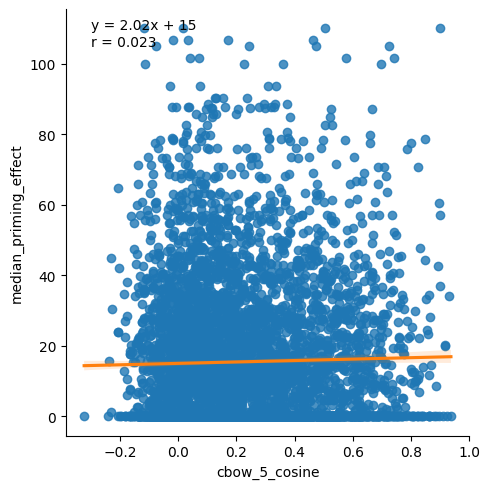
\includegraphics[width=0.45\textwidth]{images/cbow_5_cosine_against_priming_effect.png}
    \caption{A scatter plot of the cosine similarities of prime-target pairs generated by the CBOW Window 5 model against their median priming effects. The orange line is a linear regression between the variables, whose formula and Pearson correlation coefficient is given in the upper left corner.}
    \label{fig:cbow_5_cosine_against_priming_effect}
\end{figure}

The full results of the second analysis can be found in the appendix of this report.
For now, I will look at the results of the CBOW Window 5 model as a baseline, but all results are very similar across models.
Figure \ref{fig:cbow_5_cosine_against_priming_effect} shows the cosine similarities of the CBOW Window 5 model against the semantic priming effects of prime-target pairs.
From these results, I was unable to find any proof that cosine similarities are good predictors of priming effects.
There seems to exist no clear relationship between cosine similarity and priming effect size: not only are the regression models clearly incapable of modeling a linear relationship between the variables, but from human intuition and insight, I am also unable to find any clear relationship between the variables.
The data in the scatter plots seem very varied, and only one big cluster of data.
Although not included in the results, I also performed this analysis with negative priming effects.
This resulted in plots where the relationship between the two variables seemed to be non-existent, just like in figure \ref{fig:cbow_5_cosine_against_priming_effect}, the only difference being that the independent normal distribution of both variables could be easily observed.

After finishing the analyses, I constructed distributions of the cosine similarities generated by the word2vec models.
The distribution of cosines generated by the CBOW window 5 model is shown in figure \ref{fig:cosine_cbow_5_distribution}.
I found that all models roughly share this distribution: normally distributed around 0.1 with a positive skew.
This corroborates my expectations: high similarities should occur infrequently, and low similarities should occur frequently, since every word only has a handful of other words that are semantically related to it.

\begin{figure}
    \centering
    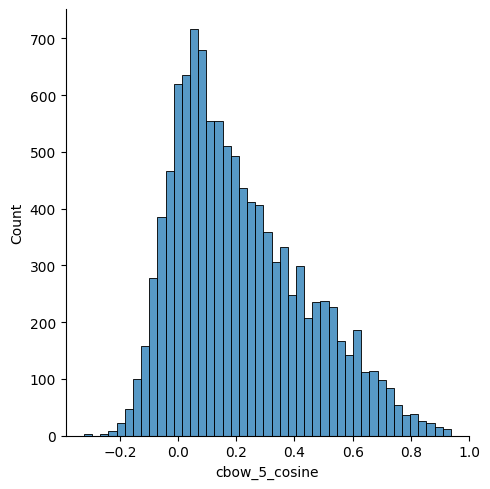
\includegraphics[width=0.45\textwidth]{images/distribution_cbow_5_cosine.png}
    \caption{A plot of the distribution of all cosine similarities of prime-target pairs generated by the CBOW window 5 model.}
    \label{fig:cosine_cbow_5_distribution}
\end{figure}

\section{Conclusions}
For the first experiment, I would conclude that semantic relatedness levels and cosine similarities align.
All models clearly show that a higher semantic relatedness of a prime-target pair results in a higher mean cosine similarity.

For the second experiment, I would conclude, for the data analyzed and the models used, that, irrespective of model hyperparameter values, cosine similarities are not a good predictor of priming effect size.
The relationship between the two variables seems to be non-existent, both being independently normally distributed.

\end{document}